\documentclass[journal]{IEEEtran}

\usepackage{cite}
\usepackage{amsmath}
\usepackage{verbatim}
\usepackage{multirow}
\usepackage[unicode,pdftex]{hyperref}

\usepackage{xcolor}


\ifCLASSINFOpdf
\usepackage[pdftex]{graphicx}
\else
\fi

\hyphenation{op-tical net-works semi-conduc-tor}

\newcommand{\reffig}[1]{Fig. \ref{#1}}
\newcommand{\refsec}[1]{Section \ref{#1}}
\newcommand{\refeq}[1]{Eq. \ref{#1}}
\newcommand{\reftab}[1]{Table \ref{#1}}

\newcommand{\tabincell}[2]{\begin{tabular}{@{}#1@{}}#2\end{tabular}}

\DeclareMathOperator*{\argmax}{argmax}
\DeclareMathOperator*{\argmin}{argmin}


\definecolor{level2}{RGB}{255,255,255}
\definecolor{level3}{RGB}{10,10,10}
\definecolor{revised}{RGB}{100,101,140}
\definecolor{continue}{RGB}{255,0,0}
\definecolor{filltext}{RGB}{0,255,255}

\begin{document}
\title{Background Subtraction based on Deep Feature Transformation Learning Background Subtraction}

\author{Xinyu Ren,
        Chenqiu Zhao,
		Yongxin Ge }


\maketitle


\begin{abstract}
% 背景建模是一个复杂的问题
Background subtraction is a fundamental problem of computer vision.
% 为什么复杂
The main challenges of background subtraction comes from the diversity and the complexity of natural scenes.
% 以前的工作是怎么做的
Plenty of previous works are proposed to handle this problem by artificial model.
% 我们是怎么做的
%Previous works in this field were proposed by designing an artificial model, 
In this paper,
we propose a self-adaption solution with the utilization of convolutional neural networks, 
and a novel background subtraction model named Deep Feature Transformation Learning is proposed.
% 动机是什么
With the motivation of finding a new representation of pixels’ historical observations in a new feature space.
% 怎么做的 XXX 这两句话介绍方法,但我实在是看不懂,你再改改
% We conduct our training and prediction processes on block level.
The videos are divided into image blocks, which are later transformed into the pixel’s observation patches.
Moreover, these patches are taken as the input of a Fully Convolutional Network(FCN). 
With the strong learning ability of FCN, we can finally get a new representation from raw RGB data, which is easier for the classification.

The architecture of the FCN proposed in this paper is devised from the semantic segmentation problem.
% 效果好
Comparisons with several state-of-the-art algorithms in well-known benchmark show the superiority of proposed approach.
\end{abstract}

\begin{IEEEkeywords} 
    Background Subtraction, Feature Transformation, Deep Learning,
\end{IEEEkeywords}

\IEEEpeerreviewmaketitle

\section{Introduction}
% introduction 的第一段介绍这个问题为什么有做的意义
% 这个问题的意义
Background subtraction or foreground object detection is a fundamental problem of computer vision, 
which has been developed over the last few decades.
% 难点在哪
The main challenges of this problem comes from the diversely natural scenes,
such as the illumination variation \cite{2017_REVIEW_7914756}, wrapping tree \cite{2014_CVIU_SOBRAL20144} and running water \cite{Bouwmans2014}.
% 现状是什么
Previous work already achieve well performances in the scenes with low complexity.
% 现有的方法是怎么做的
In particular,
a large numbers of studies are focus designing artificial model according to the characteristic of a particular scenes.
% 效果如何
Example, the multiple background model are proposed for dynamic background,
and the texture are used to handle the shadow of objects.
% 为什么这个问题还有做下去的意义
However, in view of the continuous growth in videos obtained from diversely natural scenes,
more challenging scenes are proposed for background subtraction.
% 总结,这个问题很难,还能做
It remains a challenging problem to proposed a general solution for background subtraction in all exist and potential scenes.
%
% 
% 
% robust background 
% 
% via moving cameras
% in recent years, the matter of background subtraction for
% moving cameras has attracted sustained levels of interest from
% researchers
% 
% It is widely used as the pre-processing step of video processing, which can help us efficiently mark the region of interest, e.
% vehicles and humans, thus saving us huge amount of computing resources.
% Typically, Background subtraction is a binary classification task that assigns each pixel in a video sequence with a label, for either belonging to the background or foreground scene.
\begin{figure}[!t]	% FIGURE: figure/fig1 
\centering
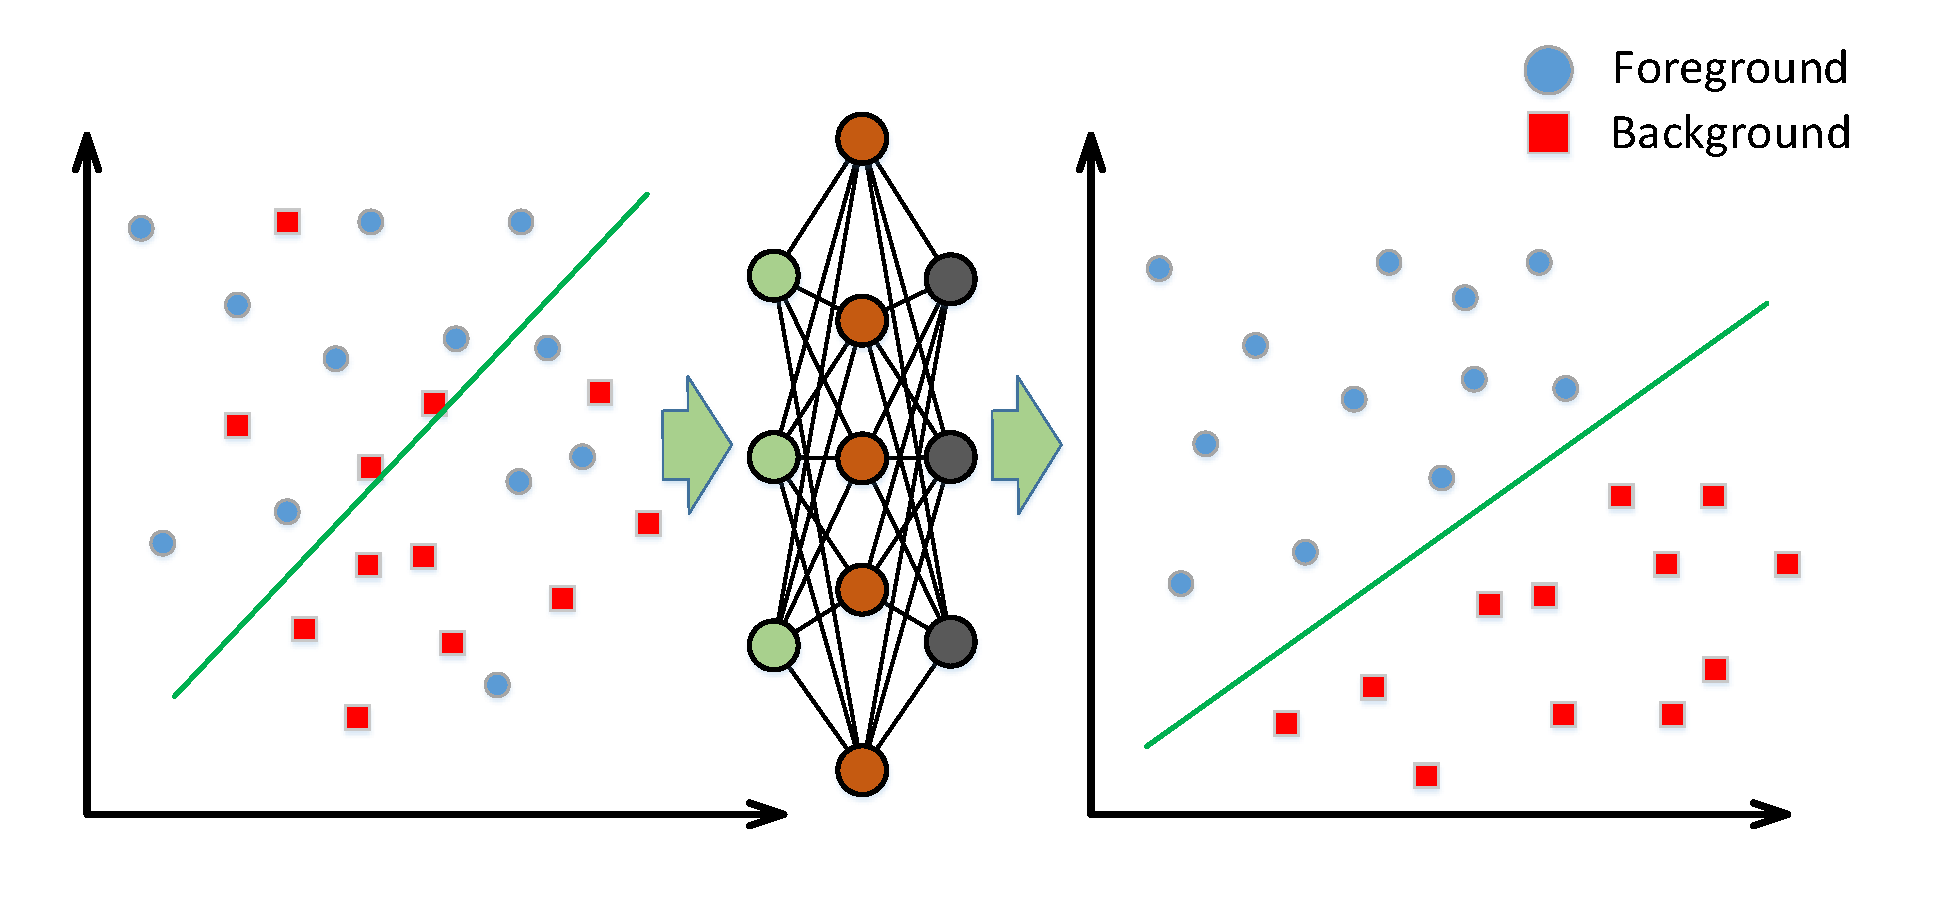
\includegraphics[width=.5\textwidth]{figure/fig1}
\DeclareGraphicsExtensions.
    \caption{The illustration of Proposed approach}
\label{fig_FBMS_nobk}
\end{figure}


% With a huge number of works, existed algorithms have already achieved well performances in the scenes of low diversity or complexity, such as the indoor scenes.
% However, background Subtraction is still unsolved because of the diversity in background scenes and the changes originated from the camera itself.
% Scene variations can be in many forms such as, camera jitter, dynamic background, bad weather, illumination changes, intermittent object motion.
% for instance, the earlier Frame Difference Methods, trying to get a fixed image as background to classify each pixels.
% The fundamental problem lies in that linear classifier might not be powerful enough for the job, due to the complexity and the diversity of natural scenes.
% 第二段介绍你的解决思路

% 说明问题的本质是什么 
Typically, Background subtraction can be viewed as a binary classification, where pixels in video stream are divided into two
types, either foreground or background.

% 以这个本质为基础来评价现存方法
With a huge number of works, existed algorithms have already achieved well performances in the scenes of low diversity or complexity,
such as the indoor scenes. However, those performance on real-world scenes like dynamic background, bad weather, illumination changes,
intermittent object motion are still not satisffied.

% 现存方法失败的原因是什么
This is principally because the major methods, in most cases, try to find a universal solution by generating some universal 
background models for later linear classification; for instance, the earlier Frame Difference Methods, trying to get a fixed 
image as background to classify each pixels. The fundamental problem lies in that linear classifier might not be powerful enough for the job,
due to the complexity and the diversity of natural scenes.

%我们的方法针对这个原因怎么样了
In order to present a better and universal solution, we proposed the Deep Feature Transformation Learning model for Background Subtraction 
in complexly natural scenes.

% XXX 为什么效果会好,同时也是我们方法的创新点, 最重要的还要结合图来说,
With the strong learning ability of FCN, we can easily get a new representation of pixels' historical observations which are much easier and clearer to distinguish.

% 总结方法的思路
In our method, the main job is to transform the sequence of pixels into another sequence which is easy for classification.

% sq1 = {p_1,p_2,...p_n} -> sq2 = {f_1,f_2,...f_n}                     (1)

For sq1, it is a sequence of pixels' intensity, which is hard to classify which entry is foreground or background.
But in sq2, it is more easy to classified, since the output of the network is the label of each entry in sequence.

% 第三段介绍具体是怎么做的
More particularly, videos are divided into image blocks at the beginning. Then, pixel's observation patches are extracted from these blocks and sent to a FCN.
The FCN will learn and transform these patches into prediction patches where pixels are clearly for classification.
% 首先一句到两句,最多3句话总结你的方法的过程

% 补充方法的细节
In this paper, pixel’s observation patches are proposed to describe the historical observation of pixels and also as the input of our network. 
A random initialized FCN network is trained to learn the historical observation of pixels and generate a new representation in a new feature space.

% 这些细节带来的好处
We take advantage of the strong learning ability of FCN to learn a new representation of the Pixel’s observation patches in a new space where 
the pixels can be easily classified to background and foreground. 

% 最后整个list把方法的contribution 列出来
The contribution of proposed approach are summarized as follows:
(1) We present the Pixel's observation patches which give us the ability to process the pixel's historical observation with a FCN.
(2) We present a novel FCN architecture for Background Subtraction.
 
\begin{itemize}
    \item    
        % 以前怎么做的
        Most existed methods are based on Background models. 
        Unlike previous Background model based algorithms, we focus on the pixels stream itself, trying to find a space where the new representation
        of pixels are easier to distinguish. 
        % 我们这么做有什么好处
        The reason why we choose this way for the job is because we can't find a perfect background model which can adapt to all kinds of nature 
        scenes and various tasks. In this condition, we avoid to build a universal background model. And the experiment shows a good performance 
        compared with some state-of-art methods.

        % 为什么要reshape 
    \item The observations in a particular pixel are reshaped into blocks, that's because our network needs fixed size input, we also tried different 
        size of input.
        % 这么做额目的是什么,好处什么
\end{itemize}
%XXX introduction 里最好不要出现公式
\begin{equation}
    sq_1 = \{p_1,p_2,\cdots, p_n\} -> sq_2 = \{f_1, f_2, \cdots, f_n\}
\end{equation}
For $sq_1$, it is a sequence of pixels' intensity, which is hard to classify which entry is foreground or background.
%
But in $sq_2$, it is more easy to classified, since the output of the network is the label of each entry in sequence.


\section{Related Work}
%  XXX 我觉的针对方法使用的特征对方法分类比较容易。例如颜色特征,纹理特征,时空间特征,最后引出你的,特征转换
Over the last few decades, Background subtraction has been well studied. Meanwhile, a huge number of methods were proposed. These methods can be broadly categorized into pixels-based, region-based, frame-based and Deep Learning.

\subsection{A. pixels-based methods}
\label{sec_spa}
% 把你想引的论文都贴上,太多了,而且你的Zhi Zeng et al. 是tm的谁啊??
The most widely used algorithms in Background subtraction are pixels-based methods.
And one of the famous method is Gaussian Mixture Model (GMM) \cite{Zivkovic2004}, in which a GMM is used to model the history over time of pixel’s intensity values.
It is assumed that pixels are independent from their neighbors.
Incoming pixels are labeled as background if there exists a Gaussian in the GMM, where the distance between its mean and the pixel lies within a certain bound.
For learning the parameters, that maximize the likelihood, the authors proposed an online method that approximates the Expectation Maximization (EM) algorithm.

In XXX , Mingliang Chen et al.\ \cite{2017_TPAMI_GANGWANG} propose a background subtraction algorithm using hierarchical super-pixels segmentation, spanning trees and optical flow.
Their Background model combine the GMM with constrains of temporal and spatial from optical flow and super-pixels \cite{6205760_2012_TPAMI}.

Kim et al.\ \cite{Kim2004} used a codebook to record the sampling background values at each pixel, which can be seemed as a compressed representation of background model.
This allows them efficient in memory and speed compared with other background modeling techniques.
The final foreground is detected by a distance measurement in a cylindrical color model.

In XXX, Zhi Zeng et al.
proposed an equal-qualification updating strategy to replace the maximum-negative-run-length-based filtering strategy.
Their experiments show that, the proposed method outperforms well, despite using only color information.

Elgammal et al.
introduced a probabilistic non-parametric method to model the background.
It is assumed that each background pixel is drawn from a PDF.
The PDF for each pixel is estimated with Kernel Density Estimation (KDE).
\label{sec_geo}
region-based approach assumpt that the neighbouring pixels have a similar variation as the pixel itself.

In xxx, Sriram Varadarajan et al.
propose a region-based MoG to takes in which the updated mixtures represent the scene distribution in a neighbourhood region.

In (PCA), classification is done by comparing a block in current frame to its reconstruction from PCA coefficients and declaring it as background if the reconstruction is close.

A recently region based method is presented in XXX which used the statistical circular shift moments (SCSM) in image regions for change detection.

subspace learning method in xxx, is used to compress the background into the eigenbackground.
For each video, the mean and the covariance matrix are calculated.
After a PCA of the covariance matrix, a projection matrix is set up with M eigenvectors.
Then, incoming images are compared with their projection onto the eigenvectors.
Foreground labels are assigned to pixels with large distances, after calculating the distances between the image and the projection and comparing them with the corresponding threshold value.

Marghes et al.
used a mixed method that combines a reconstructive method (PCA) with a discriminative one (LDA) to robustly model the background.

single Gaussians are employed for foreground modeling.
By computing flux tensors, which depict variations of optical flow within a local 3D spatio-temporal volume, blob motion is detected.
With the combination of the different information from blob motion, foreground models and background models, moving and static foreground objects can be spotted.
Also, by applying edge matching, static foreground objects can be classified as ghosts or intermittent motions.

Frame-based background modeling via Principal Component Analysis (PCA) and low-rank/sparse decomposition approaches is a popular alternative to pixel-level modeling xx.
These approaches are however not ideal for surveillance applications as most rely on batch or offline processing or suffer from scaling problems.

In XXX, ss et al.
addressed scaling problems by reformulating principal component analysis for 2D images.
Meanwhile their method takes much lower memory consumption and computational cost than others.
Some online approaches have also been proposed recently, but they are still very computationally expensive.
\label{sec_sup}
A novel approach for background subtraction with the use of CNN was proposed by Braham and Droogenbroeck.
They used a fixed background model, which was generated from a temporal median operation over N video frames.

In XXX, Yi Wang et al.
tried a CNN architecture combined with a Cascade model for segmentation in Background subtraction.
Given 200 labelled images as training set, their model performed excellently in dataset2014.

Braham et al.
present an Deep learning-based method.
with the help of CNN, they generated a fixed background model from a temporal median operation over N video frames.
Then, a scene-specific CNN is trained with corresponding image patches from the background image.

In xxx, M.
Babaee et al.
combine the segmentation mask from SuBSENSE algorithm and the output of Flux Tensor algorithm, which can dynamically change the parameters used in the background model based on the motion changes in the video frames.
They also used spatial-median filtering as the post processing of the network outputs.



\section{The  Framework}
\label{sec3}
In this section, we introduce our DPVL model that consists of a pixels-based observation patches and a novel FCN networks for background subtraction.
We explain the details of the procedures of capturing the observation patches and the architecture of network in our DPVL model.
The complete system is illustrated in Figure XXX.
We use a set of input and ground true images to generalize the Pixels’ Variation Permutations, and reshape them into fixed-size image patches as and fed into a FCN.
After reassembling the patches into the complete output frame, it is post-processed, yielding the final segmentation of the respective video frame.

\subsection{A. Image blocks to observation  patches}
\label{sec3_fc}
The historical observations of pixels which belong to the background are usually share a common variation pattern.
In more specific terms, the variations of pixels in background are generally keeping in some pattern.
And we want to use a FCN network to learn a new representation of pixels’ observations in a new feature space.
  
In order to get enough pixels’ observations, we conduct our experiment on block-level.
In this paper, we divide each video into smaller image blocks, which share a common frame length of t.
For each image blocks, it contains M*N pixels’ historical observations in a temporal sequence of t frames.
We need to take them out for later transformation as our network input.

Observation patch is purposed to take advantage of the strong learning ability of the FCNs.
And what we need is an pixel-to-pixel transformation.
More precisely, Every historical pixels’ observation in these observation patches has an corresponding transformation  at the last layer of FCNs.
Here is how we get these observation patches.
First, we transform each image block into M*N pixel’s observation series which are the  single pixels’ historical observation series in a frame length of t.
Next, we reshape the observation sequence into a rectangle image which size is $\sqrt{t}\cdot \sqrt{t}$.
That rectangle image is what we called observation patch.
The observation patches are taken as network training sample set.

Another conception about observation patches is interval sampling.
For a sequence like this: 
\begin{equation}
    p_t\{p_1,o_2,\cdots,p_n\} -> \{p_1,p_{11},p_{21}, \cdots, p_n\}
\end{equation}
where $t$
denote the sequence number of frames.
By this way, we can get an new sequence contains more temporary information  than the continuous pixel sequences.
This works well when it comes to some situation where the moving objects keep stationary for a long time.


 
\subsection{Fully Convolutional Network}
\label{sec3_bc}
The primary task of our network is to learn an optimal feature transform of pixel’s observation series, thus we can find a new representation which is easy for classification from raw RGB data.
There needs to be a consistent one-to-one match between pixels’ observation sequence and our network output on the time series. In these circumstances, traditional convolutional network cannot meet our requirements. 
Different with those traditional ones, fully convolutional networks can take input of arbitrary size and produce correspondingly-sized output with efficient inference. 
FCNs have already been used in many areas like sematic segmentation and so on. Researchers found FCNs has a strong learning ability which won’t lost to the traditional ones, 
meanwhile, it also has a high efficient computation ability.   
FCNs utilize 1*1 kernels to take the place of fully connected layers. 
Therefore, we take a fixed size of pixel’s observation patches as the input of our network. For the convenience of calculations, we transform observation sequence into observation patches.

\subsection{Network Architecture}
The architectures of our proposed FCN is illustrated in Figure xx, our network contains 5 convolutional layers, 2 pool layers and a convolutional layer which have a filter size of 1*1.
A short calculation revealed that the network output will less 10 pixels after forward calculating.
In order to make output the same size as input, we borrowed ideas from Image semantic segmentation, which is doing zero-padding before the training.
After the forward computing, we can get the new representation of input observation values in a new feature space.
Then, after some thresholding calculations.
Our experiment results show that a random initialized FCNs, trained end-to-end on feature learning can achieve the state-of-the-art without further machinery.




\section{Experiments}
Our experiments are conducted on the computer with Nvidia tasela K20c GPU.
 And the DeepLearning tool we use is the matconvnet-23.
4 beta.

Our FCN network is random initialized, and the training epoch is set to 20.
For each video, we divide it into image blocks, which have a fixed frame length of 144.
For each image block, M*N pixel’s historical observations were taken out, where the M and N denoted the size of images.
After a simple transformation, we can get M*N pixel’s observation patches.
Each of them contains the historical observation of a pixels in a frame length of 144.

For each video, we take only one image block to generate the observation patches as our training sample set.
The other image blocks are saved for testing.

In dataset2014, most of the videos have a number of frames over 1000, thus our training data only accounts for 5% of total dataset.
But we can still get plenty of training data cause the number of the training set based on the size of images.
For example, in the video Highway of dataset2014, the image size is 320*240, so the number of observation patches for training is 76800.
In our experiment, the finally result would be better if we slightly magnify the observation patches.
We do the same to label data, but with no 0 padding.

\subsection{Evaluation Metric and Dataset}
The subjective results of background modeling approaches based on the foreground detection binary maps.
And the general international standards is F-Measure.
F-Measure is defined as:

\begin{equation}
    F=\frac{precision \dot recall}{precision - recall}
\end{equation}
\begin{figure}[!t]	% FIGURE: figure/fig1 
\centering
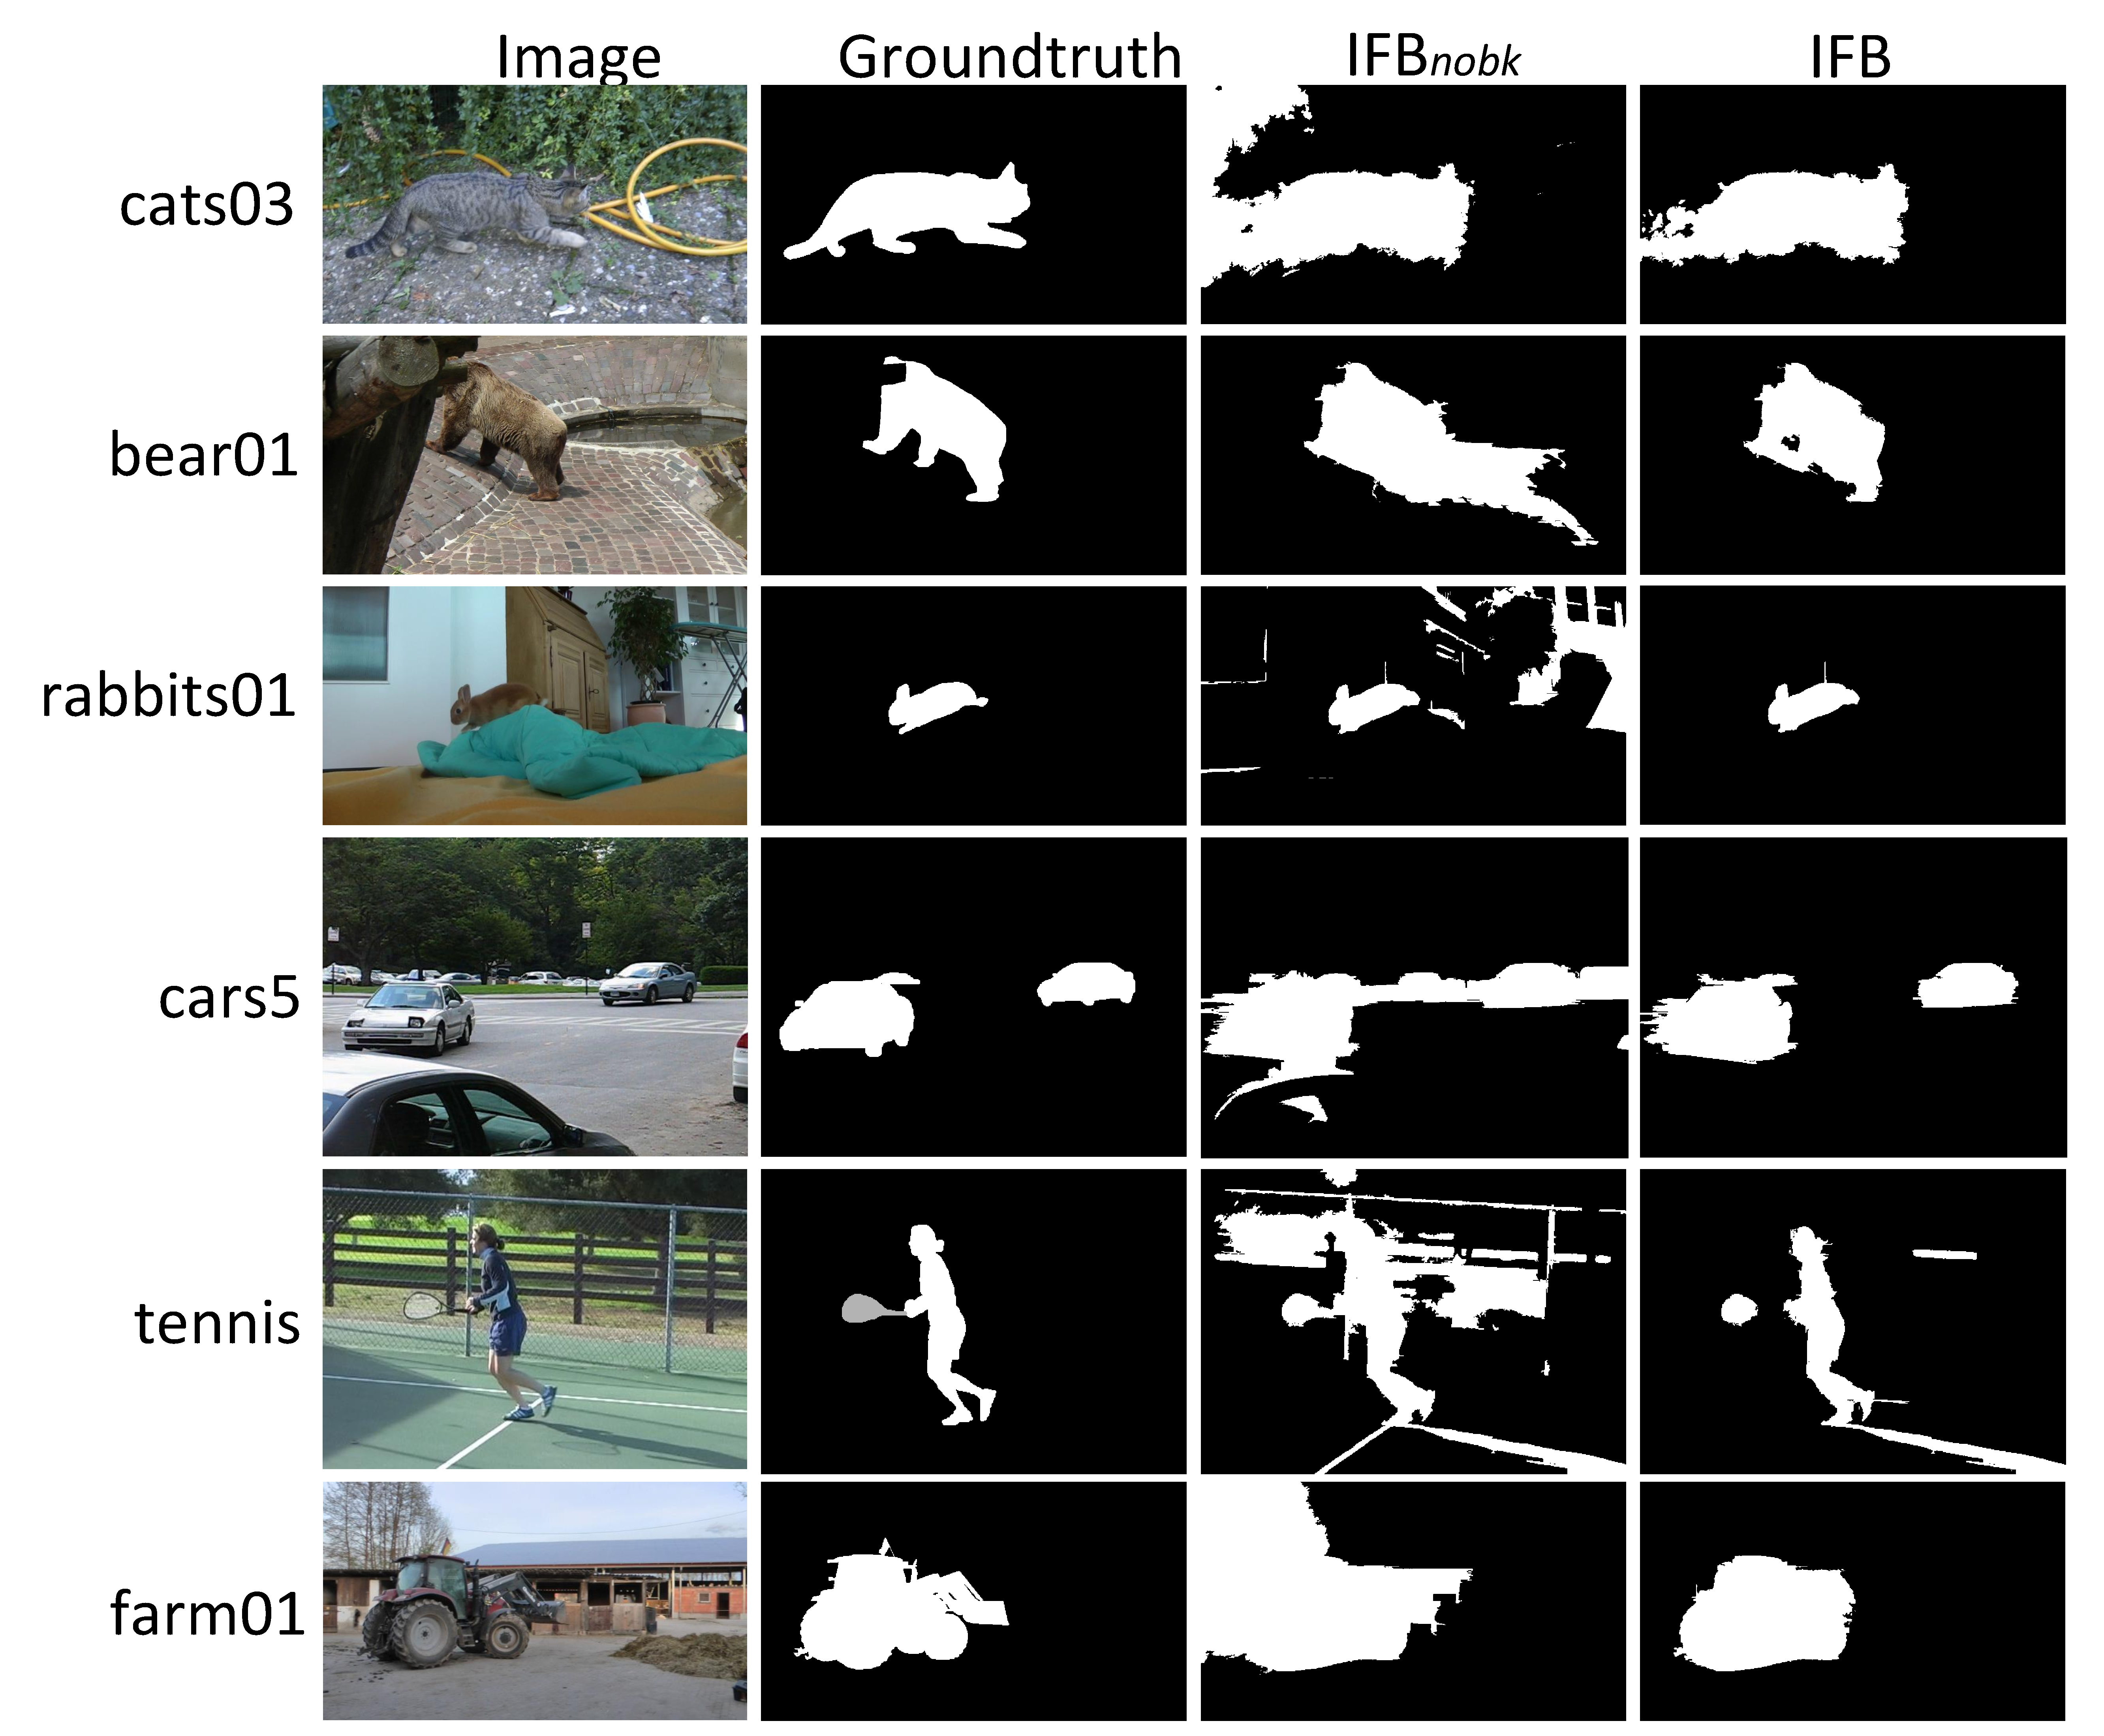
\includegraphics[width=.5\textwidth]{figure/fig_roc_fg}
\DeclareGraphicsExtensions.
    \caption{The example of latex figure.}
\label{fig_FBMS_nobk}
\end{figure}

\begin{table}[!t]				% TABLE
    \caption{The example of latex table}
\label{tab_FBMS_nobk}
\centering
    \begin{tabular}{|l@{  }c@{  }c@{  }cc@{  }c@{  }c@{  }c|}
\hline
     \multirow{2}{*}{Videos} & \multicolumn{3}{c}{$\text{IFB}_{nobk}$} &  & \multicolumn{3}{c|}{IFB} \\
    \cline{2-4} \cline{6-8}
       & Re &Pr & Fm &  &  Re & Pr & Fm  \\
\hline
cats03          &   (\textbf{0.9472} ,\   &  0.5428 ,\  &   0.6901 )   &  &    (0.9063 ,\	 &  \textbf{0.7955} ,\	 &  \textbf{0.8473} )   \\
bear01          &   (\textbf{0.9854} ,\   &  0.4806 ,\  &   0.6461 )   &  &    (0.8695 ,\	 &  \textbf{0.8673} ,\	 &  \textbf{0.8684} )   \\
rabbits01       &   (\textbf{0.9530} ,\   &  0.4433 ,\  &   0.6051 )   &  &    (0.9510 ,\	 &  \textbf{0.8730} ,\	 &  \textbf{0.9103} )   \\
cars5           &   (\textbf{0.9887} ,\   &  0.3693 ,\  &   0.5378 )   &  &    (0.9437 ,\	 &  \textbf{0.7108} ,\	 &  \textbf{0.8109} )   \\
tennis          &   (\textbf{0.9364} ,\   &  0.4558 ,\  &   0.6132 )   &  &    (0.8808 ,\	 &  \textbf{0.7345} ,\	 &  \textbf{0.8010} )   \\
farm01          &   (\textbf{0.9887} ,\   &  0.3897 ,\  &   0.5591 )   &  &    (0.8954 ,\	 &  \textbf{0.7462} ,\	 &  \textbf{0.8140} )   \\
\hline                                                                                                           
Average         &   (\textbf{0.9666} ,\   &  0.4469 ,\  &   0.6086 )   &  &    (0.9078 ,\    &  \textbf{0.7879} ,\   &  \textbf{0.8420} )   \\
\hline
\end{tabular}
\end{table}

% Videos & GBSSP\cite{Lim2014_2014_ECCV} & calMoSeg\cite{2016_ECCV_Bideau2016}  & MLayer\cite{2017_ICCV_zhu2017multilayer}  & $\text{IFB}_{SU}$ & $\text{IFB}_{KA}$ & $\text{IFB}_{SI}$ & Videos & GBSSP\cite{Lim2014_2014_ECCV} & calMoSeg\cite{2016_ECCV_Bideau2016} & MLayer\cite{2017_ICCV_zhu2017multilayer}  &  $\text{IFB}_{SU}$ &  $\text{IFB}_{KA}$  &  $\text{IFB}_{SI}$  \\
\section{Conclusions}
In this paper,
we proposed the framework for background subtraction for the case of pixels' historical observation.
Unlike previous work in which attempts were made to improve the accuracy of the estimation of motion,
our method focuses on transform the foreground cues for Background Subtruction.
In particular, 
pixels' historical observations are obtained from image blocks with the estimation of background motion,
% the geometric constraints between the SIFT features.
Then, super-pixels under multiple levels are utilized to integrate these cues.
The efficiency of historical observation from the complementarity between foreground and background cues.
A comprehensive experiment to compare our results with the state-of-the-art shows the efficiency of our framework and points to its potential for use in practical applications.

\ifCLASSOPTIONcaptionsoff
  \newpage
\fi

\bibliographystyle{IEEEtran}  
\bibliography{ref}  


\end{document}
